\documentclass[a4paper,12pt]{article}
\usepackage[utf8]{inputenc}
\usepackage{graphicx}
\graphicspath{ {img/} }

\setlength{\oddsidemargin}{0mm}
\setlength{\evensidemargin}{-14mm}
\setlength{\marginparwidth}{0cm}
\setlength{\marginparsep}{0cm}
\setlength{\topmargin}{2mm}
\setlength{\headheight}{0mm}
\setlength{\headsep}{0cm}
\setlength{\textheight}{240mm}
\setlength{\textwidth}{168mm}
\setlength{\topskip}{0mm}
\setlength{\footskip}{10mm}
\setlength{\parindent}{8ex}

\begin{document}
	\begin{titlepage}
    		\begin{center}
        		\vspace*{1cm}
        
        		\textbf{ENEL403  State-space design for an inverted pendulum and 3 cart controller}
        
        		\vspace{0.5cm}
        		Lab Report
        
        		\vspace{1.5cm}
        
        		\textbf{Jono Kapene \\ 53044694}
        
        		\vfill
        		
        		\vspace{0.8cm}
        
        		Group E16\\
        		University of Canterbury\\
        		15th May, 2017
        
    \end{center}
\end{titlepage}
	\clearpage
	
\section{Abstract}
\clearpage
\section{Introduction}

This report details the state space design for a inverted pendulum controller, and a triple cart controller. These controller design were first modelled and simulated in the program MatLab and then tested on the actual thing. Two controllers were designed, one using LQR method and the other and manually placing poles.The inverted pendulum was modeled using the given state space equation in the form $$\dot{X}=AX+B_1U,Y=C_1X$$.

\begin{center}
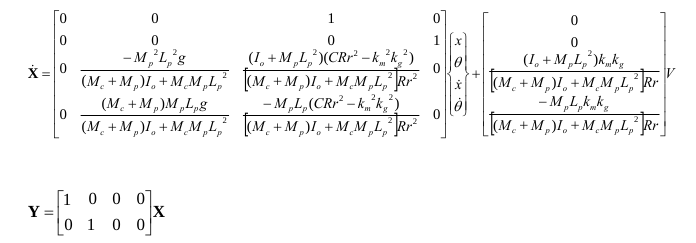
\includegraphics[scale=0.4]{iP_matrix.png}
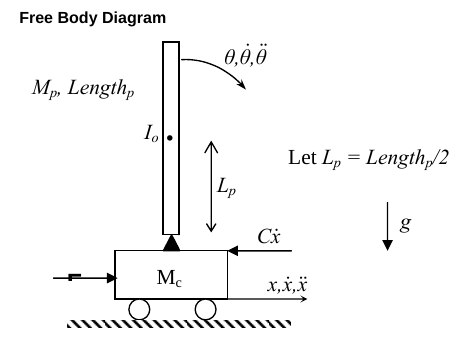
\includegraphics[scale=0.3]{iP_diagram.png}\\
\end{center}
\noindent
The triple cart system is modelled from the diagram below.
\begin{center}
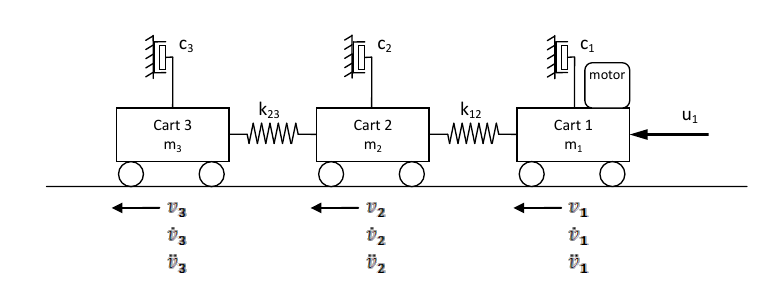
\includegraphics[scale=0.3]{3cart_diagram.png}\\
\end{center}



\clearpage
\section{Method}
\textbf{Inverted Pendulum Controller}\\
The inverted pendulum system was modeled in matlab using $ss()$ function.\\
To confirm that the system is currently unstable, the poles of matrix A are found by using the $eig(A)$ function in MatLab.To stabilize the system, feedback was introduced. For this to be possible all four states must be controllable, which was found by using the $ctrb()$ and $rank()$ functions.\\

After the system has been verified unstable and fully controllable, the controller cn now be designed. The first method used was linear quadratic regulation to determine the state feedback control gain matrix $K$. The matlab function lqr was used which parameters change the relative importance of the controller effort and error. The simpilist Q and R are chosen to find the first set of gains : $$Q = C'*C$$ $$R = 1$$ $$K = lqr(A,B1,Q,R)$$


Creating the state space equations for the new closed loop system:
$$Ac = [(A-B*K)];$$
$$B1c = [B1];$$
$$C1c = [C1];$$
$$Dc = [D];$$

By increasing the values in the Q matrix you can increase the weight the controller has on the errors at the cost of increased controller effort. The Q matrix was changed by trial and error to meet the specifications.
Once the controller has met the rest of our specifications, precompenstion(N) needs to be added to meet our steady state error requirements. Firstly the C matrix is modified so only $x$ (Cart position) is affected as there is no steady state error from $\theta$.$$CN = [1 0 0 0]$$ $$sys_ss = ss(A,B1,CN,D)$$ $$N = rscale(sys_ss,K)$$
These state space models are a simulation of the lab models and appropriate graphs are plotted below in the \emph{results} section of this report.\\
\clearpage
\noindent
\textbf{Triple Cart}\\

\section{Results}

\section{Discussion}

\section{Conclusion}


\end{document}